\section{Fabrication} \label{sec:fab}

In order to successfully identify the 2 ns electron beam bunch structure delivered by the CEBAF to within 99\% accuracy, the \gx{} Start Counter time resolution is required to be $<350\ \mathrm{ps}$.  In the following section the details of polishing and characterizing machined scintillators, as well as the construction of the Start Counter are discussed.

\subsection{Polishing Machined Scintillators} \label{sec:fab_polish}

The surfaces of the machined scintillators incurred a plethora of surface defects and chemical contaminants known to harm scintillator surfaces while undergoing edge polishing at McNeal Enterprises.  Therefore, in an effort to recover the scintillator surfaces and performance capabilities, polishing was required.

Prior to polishing the machined scintillators, a coarse measurement of the paddles performance was conducted to understand the magnitude of damage the paddles had incurred, relative to prototypes, as a result of mishandling.  The time resolution and light output was measured at three precise locations along the length of the scintillators. One measurement was taken in the middle of the straight section, one in the middle of the bend, and one at the tip of the nose. 

Figure~\ref{fig:Initial_Paddle_Prop_UW} illustrates the erratic fluctuation and poor performance that existed from paddle to paddle prior to polishing. 
	\begin{figure}[!htb]
		\centering
		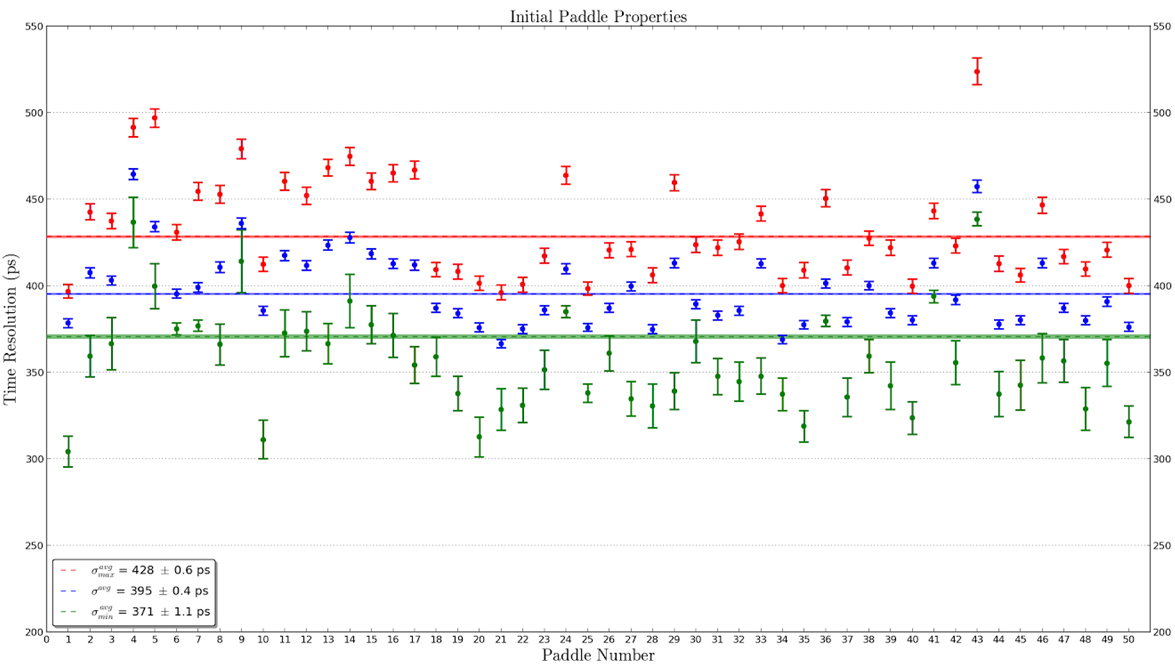
\includegraphics[width=1.0\columnwidth]{fabrication/figs/Initial_Paddle_Prop_UW}
		\caption{Coarse time resolution measurements prior to polishing. Paddle number is on the x-axis and time resolution in ns is on the y-axis. The red points are the resolutions in the bend region, the blue points are the weighted average of the three measurements, and the green points are the resolutions at the tip of the nose.  The horizontal lines are the weighted averages of the individual measurements.}
		\label{fig:Initial_Paddle_Prop_UW}
	\end{figure}
On average the 50 paddles did not meet the design resolution of 350 ps.

To polish the machined scintillator surfaces, Buehler Micropolish II deagglomerated $\mathrm{0.3\ \mu m}$ alumina suspension was utilized\cite{buehler}.  The polishing suspension was diluted with a 5:1 ratio of de-ionized $\mathrm{H_{2}O}$ to alumina and applied to a cold, wet $6'' \times 0.5''$ Caswell Canton flannel buffing wheel\cite{caswell} operated at $\mathrm{<1500~RPMs}$. All surfaces of the scintillators were carefully buffed until all large, uniform surface defects were removed. In order to eliminate small, localized surface defects hand polishing with a soft NOVUS premium Polish Mate microfilament cloth\cite{novus} and diluted polishing suspension was applied.  These polishing procedures made the scintillators void of virtually all scratches and surface defects.

Once the appropriate polishing procedures had been developed and implemented the surface quality was greatly improved as can be seen in Fig.~\ref{fig:polshing_effects} which illustrates the same scintillator paddle before and after polishing.
	\begin{figure}[!htb]
		\centering
		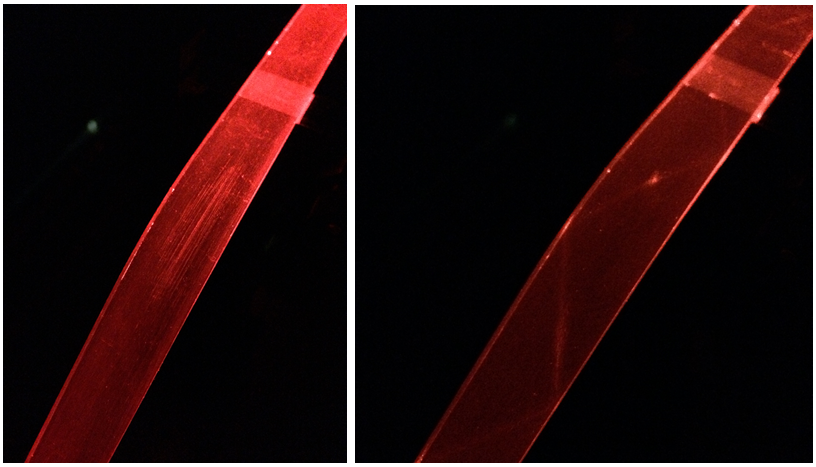
\includegraphics[width=1.0\columnwidth]{fabrication/figs/polshing_effects}
		\caption{Effects of polishing scintillators. Left: non-diffuse laser incident on an edge, before polishing, at the upstream end of the straight section. Right: non-diffuse laser incident on the same edge, after polishing, at the upstream end of the straight section.}
		\label{fig:polshing_effects}
	\end{figure}
A red laser beam was shone into the scintillator medium from the upstream end aimed at one edge so that the total internal reflection towards the tip of the nose was visible.  The unpolished scintillator had such poor surface quality that the reflections in the bend region could not be seen due to the multiple scattering of light at the scintillator boundaries.  However, the reflections in the polished scintillator can clearly be seen traversing down through the nose region.

Once the scintillators were polished, their performance was remeasured so that a quantitative measure of the polishing effects were understood.  The measurements were performed in an identical manner outlined above and the pre-polished results were illustrated in Fig.~\ref{fig:Initial_Paddle_Prop_UW}. As expected, the time resolutions were greatly improved as seen in Fig.~\ref{fig:Polished_Paddle_Prop_UW}.
	\begin{figure}[!htb]
		\centering
		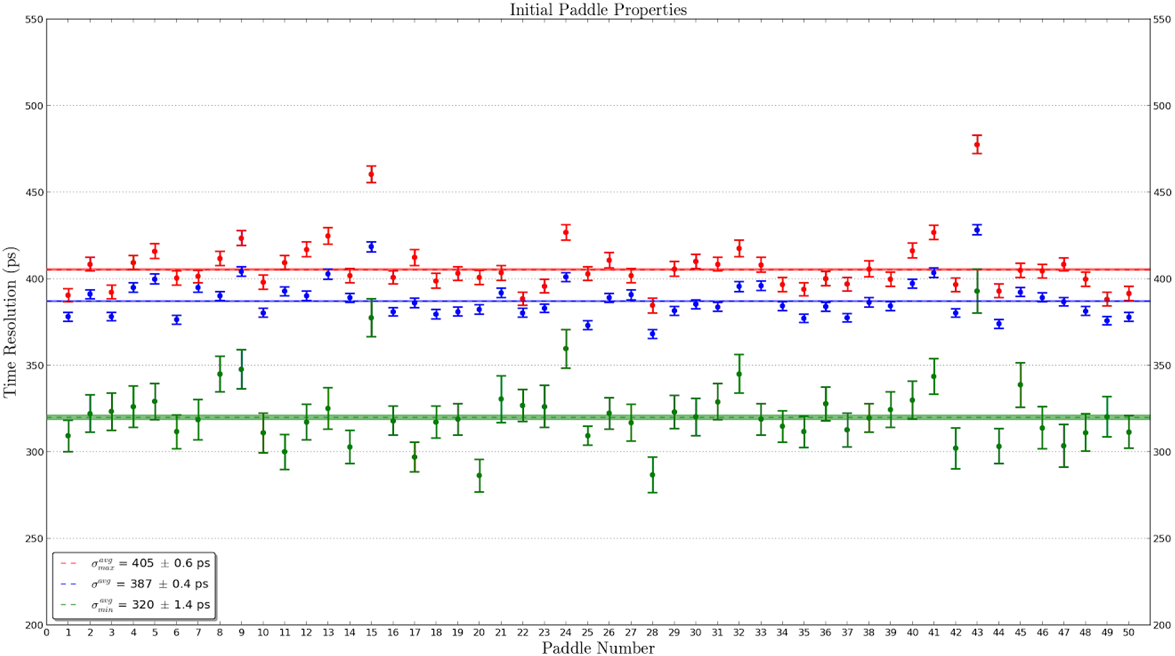
\includegraphics[width=1.0\columnwidth]{fabrication/figs/Polished_Paddle_Prop_UW}
		\caption{Coarse time resolution measurements after polishing. The details are identical to Fig.~\ref{fig:Initial_Paddle_Prop_UW}}
		\label{fig:Polished_Paddle_Prop_UW}
	\end{figure}
On average, at the tip of the nose, the scintillators exhibited a $\approx15\%$ improvement in time resolution.  Moreover, there was a substantial reduction in erratic fluctuations in performance.

\subsection{Testing Machined Scintillators} \label{sec:fab_test}

The polished machined scintillators were tested in order to measure their light output and time resolution properties.  They were measured in an identical and reproducible manner utilizing a custom fabricated test stand shown in Fig.~\ref{fig:test_stand_model}. 
	\begin{figure}[!htb]
		\centering
		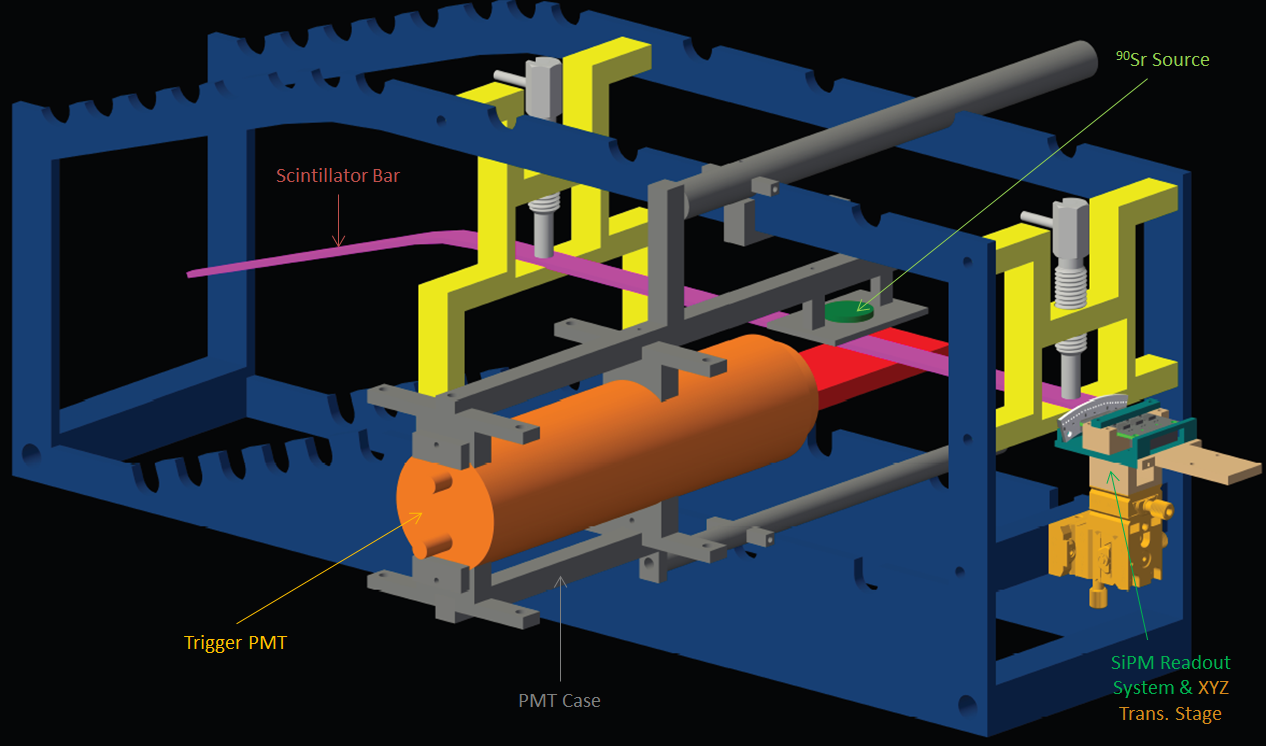
\includegraphics[width=1.0\columnwidth]{fabrication/figs/test_stand_model}
		\caption{CAD Drawing of custom test stand.}
		\label{fig:test_stand_model}
	\end{figure}
The test stand facilitated the precise measurement of the aforementioned scintillator properties at 12 well-defined locations along the length of the scintillator paddles.  Specifically 4 locations in the straight section, 3 in the bend, and 5 in the nose were tested.  

The measurements were conducted with a collimated $\mathrm{^{90}Sr}$ source oriented orthogonal to the wide flat surface of the scintillators.  The $\mathrm{^{90}Sr}$ source provided minimum ionizing electrons ranging in energy from $\mathrm{0.5-2.3~MeV}$ \textit{via} beta-decay \cite{nndc_sr90}\cite{nndc_y90}.  A trigger Photo-Multiplier Tube (PMT) was placed underneath the scintillator on the opposite side of the $\mathrm{^{90}Sr}$ source and provided the TDC start time and ADC gate.  A prototype SiPM detector identical to the SiPMs installed in the final ST assembly, was utilized to collect the light from the scintillators.  

The analog signals from the SiPM and the trigger PMT were then processed through Nuclear Instrumentation Modules (NIM) so that both the ADC and TDC spectra could be analyzed.  The signal processing electronics diagram is illustrated in Fig.~\ref{fig:nimelectronicsdiagram}.
	\begin{figure}[!htb]
		\centering
		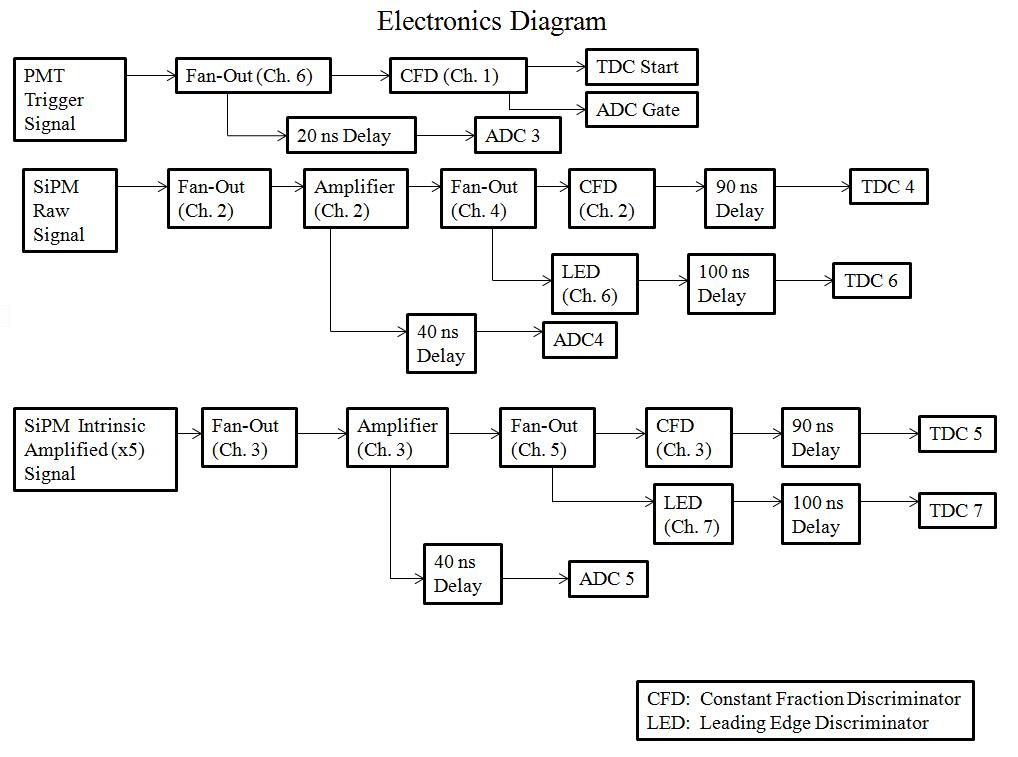
\includegraphics[width=1.0\columnwidth]{fabrication/figs/nim_electronics_diagram}
		\caption{Electronics diagram for testing machined scintillators.}
		\label{fig:nimelectronicsdiagram}
	\end{figure}

Utilizing a dedicated data acquisition computer configured with CEBAF Online Data Acquisition (CODA) software, 10,000 event triggers and associated data were collected at each of the locations along the scintillator path.  Subsequently, the ADC and TDC data were analyzed to measure the light output and time resolutions respectively of the whole lot of polished machined scintillators.  

Once the 30 machined scintillator paddles which exhibited the best time resolution and light output properties from the lot of 50 were selected, they were carefully wrapped in Reynolds food grade aluminum foil.  The aluminum foil is $\mathrm{16.5~\mu~m}$ thick and possesses good reflectivity properties.  Moreover, the aluminum foil protects the surfaces of the scintillators during both the testing and assembly processes.
  
The measured time resolutions for the 30 best scintillators, which comprise the ST, were found to be satisfactory and even well below design resolution in the nose region which is illustrated in Fig. \ref{fig:time_res_comp_final_30}.
	\begin{figure}[!htb]
		\centering
		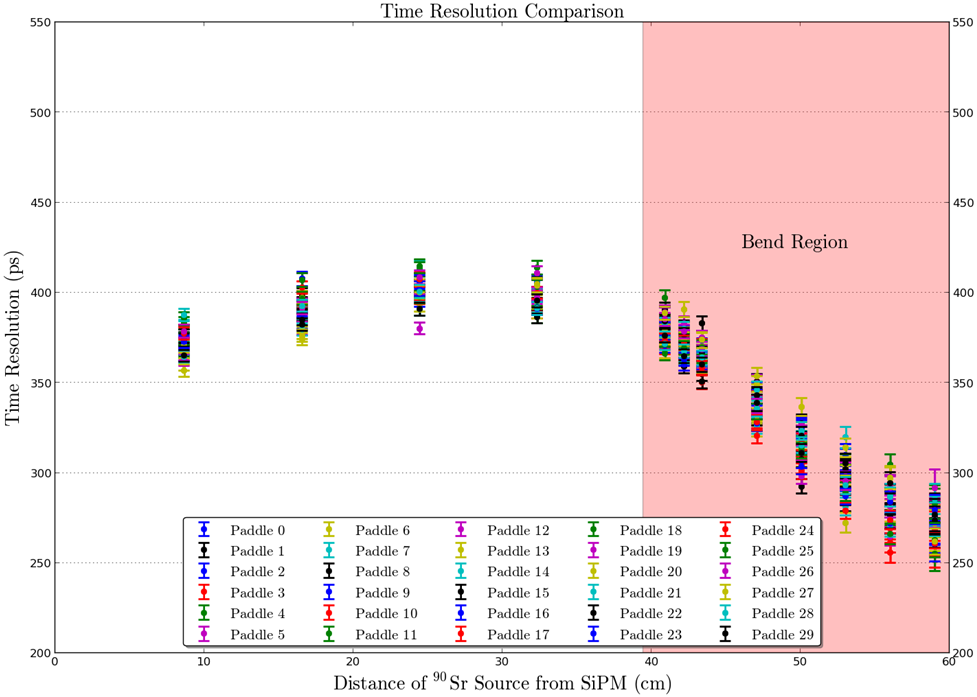
\includegraphics[width=1.0\columnwidth]{fabrication/figs/time_res_comp_final_30}
		\caption{Time resolution of 30 the best scintillator paddles.  The time resolution performance of the selected scintillators is remarkably similar while illustrating a spread of $\approx 50\ ps$ in the nose region.}
		\label{fig:time_res_comp_final_30}
	\end{figure}

The unique geometry of the machined scintillator paddles exhibit a phenomenon of an increase in light collection in the nose region as the light source moves towards the tip at the downstream end.  It is hypothesized that the relatively poor time resolution in the straight section is due to a reflective smearing effect in which light is able to traverse from the straight section down to the tip of the nose, and then back up to the upstream end.

The average time resolution of the individual scintillators selected for the final ST assembly are shown in Fig. \ref{fig:final_30_tr_wrapped}.
	\begin{figure}[!htb]
		\centering
		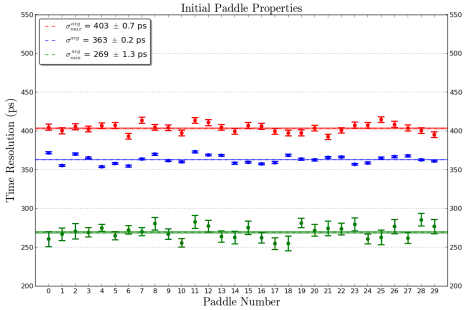
\includegraphics[width=1.0\columnwidth]{fabrication//figs/final_30_tr_wrapped}
		\caption{Average time resolution of 30 best scintillator paddles.  The red data points correspond to the maximum time resolution obtained in all 12 data points. The blue data points are the weighted average of all 12 data points.  The green data points indicate the minimum time resolution obtained in all 12 data points.}
		\label{fig:final_30_tr_wrapped}
	\end{figure}

\subsection{Assembly}

